%% The following is a directive for TeXShop to indicate the main file
%%!TEX root = diss.tex

\chapter{A new taxonomy of 3D Reconstruction}
\label{ch:3DRecon_Taxo}
Existing taxonomies of 3D reconstruction techniques generally only focus on one category of techniques: ~\citeauthor{seitz2006comparison} proposed  multiple means to classify Multi-view Stereo algorithms from various perspectives. Reviews \cite{geng2011structured, salvi2004pattern} of Structured Light techniques generally classify techniques based on the type of projection pattern used. Photometric Stereo algorithms are classified by the assumptions or generalizations made, for instance, calibrated/uncalibrated, unknown/known reflectance, unknown/known light conditions, etc. This framework provides a means to categorize intra-category algorithms, but is unsuitable to evaluate the performance of each technique across object with a range of attributes.

To have a more comprehensive understanding of the strengths and weaknesses of different techniques, a more general taxonomy is need, and one of the most popular framework categorizes 3D reconstruction techniques into active and passive methods: if the controlled light condition is used, then it's active, otherwise, it's passive. Other notable taxonomy is the spacetime framework proposed in \cite{davis2003spacetime}, which categorizes depth from triangulation techniques based on the sources of information: temporal or spatial information. Though widely adopted, the mapping of the algorithm to the conditions that works the best is generally empirical.

In the previous taxonomies, algorithms of a certain category generally work well on limited conditions, and a it's crucial to understand where algorithms perform well and where they fail. Under the previous framework, this knowledge is largely empirical, with each algorithm roughly maps to a problem domain that is poorly defined.

The taxonomy proposed in this chapter defines the 3D reconstruction techniques from a object-centered viewpoint, \ie categorize algorithm based on object class. This taxonomy transforms the 3D reconstruction problem from one requiring knowledge and expertise of specific algorithms in terms of how and when to use them, to one requiring knowledge of the visual and geometric properties of the target object.

We need to way general/univeral enough that incorporates any between-class methods, and distinctive enough that distinguish with-class methods.

\section{Object class}
In Figure~\ref{fig:obj_class}, we show a taxonomy of object classes with different material and shape properties. There are in total $3\times 3\times 4\times 2\times 5 = 360$ classes of objects, which still don't fully capture the variations exhibited by existing objects. Most techniques that have been developed over the past decades have focused on opaque objects with diffuse reflectance. However, the majority of currently available techniques can only tackle a subset of all possible classes. For instance, MVS algorithms typically work very well for diffuse texture object, while there is no robust algorithm for specular, refractive objects.
\begin{figure}[h]
\centering
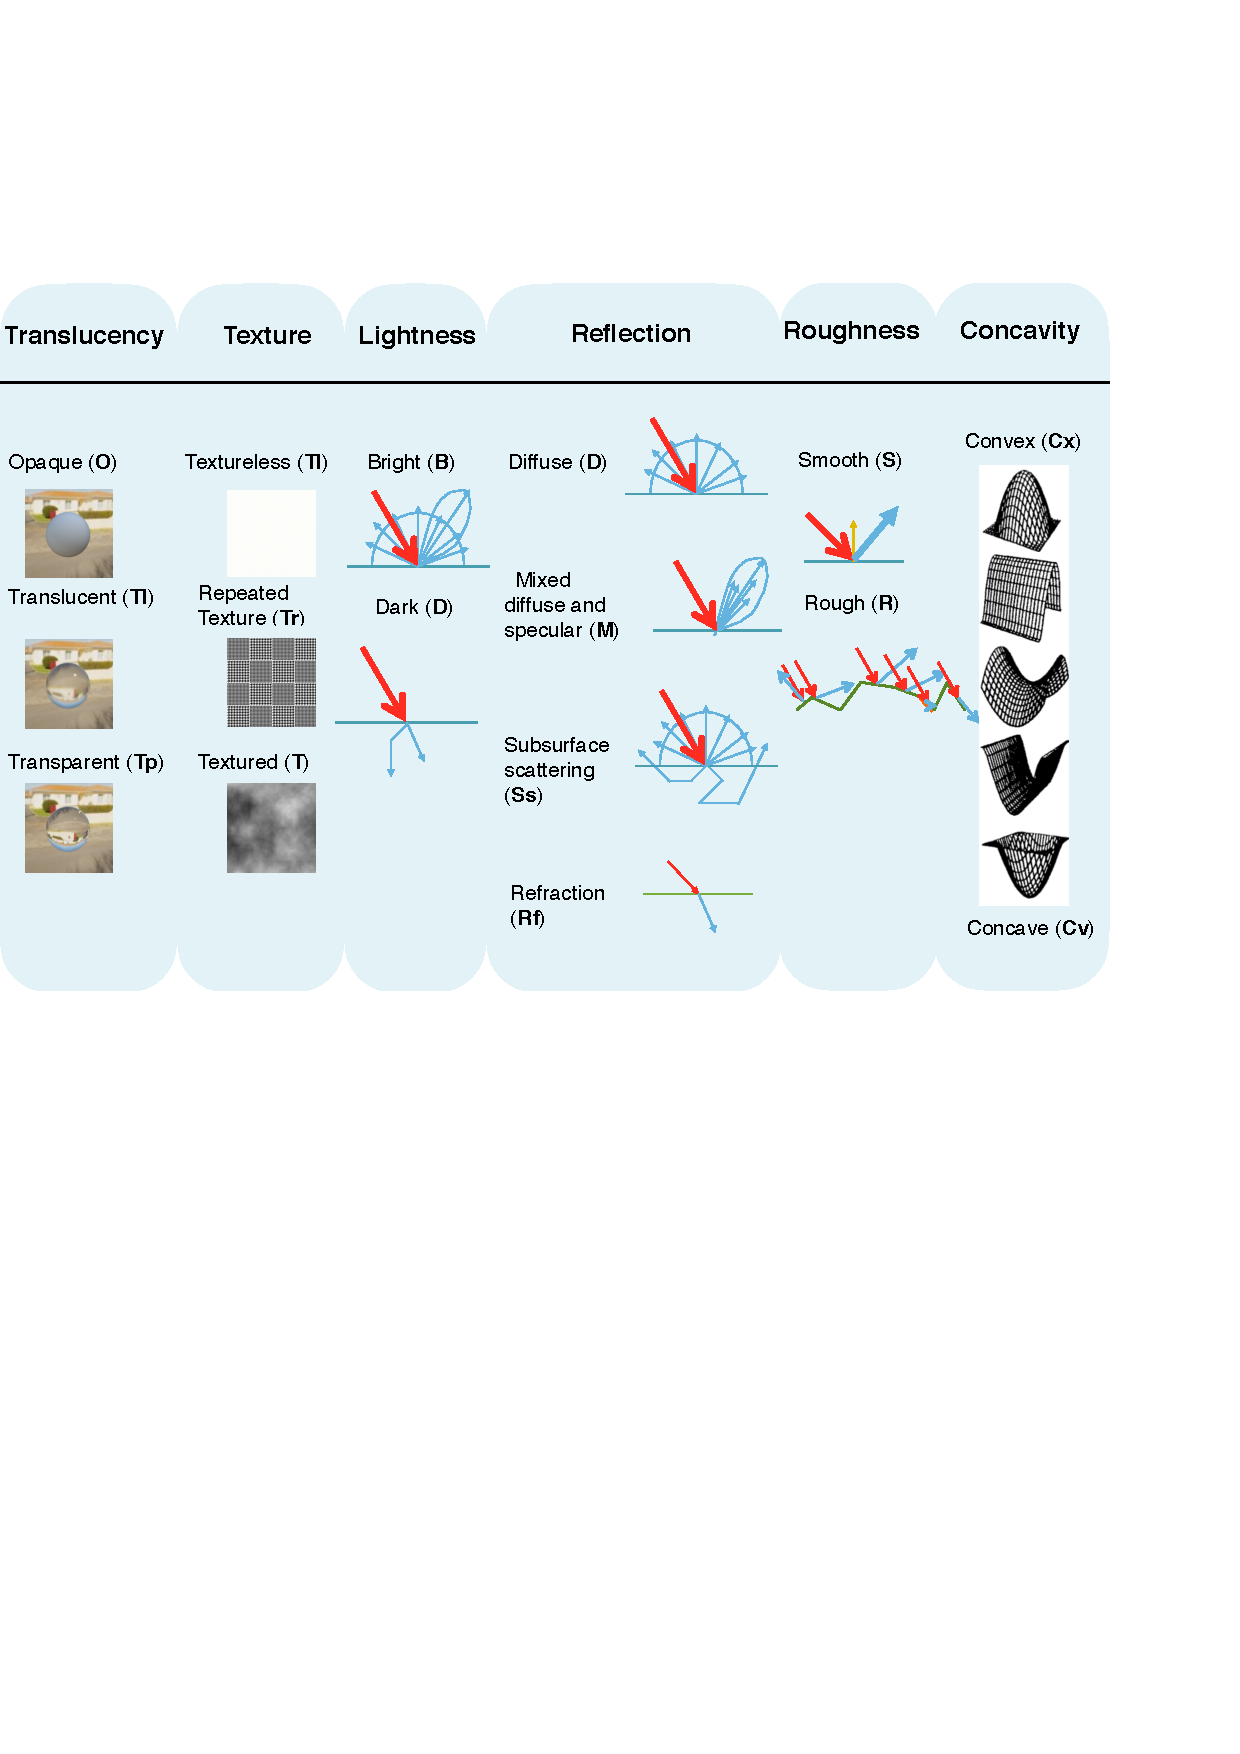
\includegraphics[width=\textwidth]{taxo/obj_class}
\label{fig:obj_class}
\caption{Object class}
\end{figure}

\section{Opaque and diffuse}
Section~\ref{sec:3DRecon_Tech} of Chapter\ref{ch:RelatedWork} discusses techniques that are best-suited for opaque and diffuse objects.

\section{Summary}
Our taxonomy focuses on the visual cues detected in images, which is utilized by various techniques. Conceptualize these visual cues as dimension of the 3D reconstruction problem, we have an abstraction which allow us to think of algorithms as volumes within a $n-$dimensional problem space. Existing algorithms can be introduced into this framework based on the main visual cue used for reconstruction. Instances where these algorithms have been reported as supporting other forms of variation have been outlined, providing an initial mapping of the space that is summarized below in Table~\ref{tab:algo_label}.
\begin{table}[h]
  \centering
  \begin{tabular}{l*{5}{c}}
  \hline
  \textbf{Technique} & Setup & Dom & Cue & Charact & Rep\\
  \hline
  PMVS & $C_n$ & $S$ & $T$ & $P$ & $P$\\
  Goesele & $C_n$ & $S$ & $T$ & $D$ & $D$\\
  Woodham & $C_1L_n$ & $T$ & $I$ & $LDS$ & $N$\\
  Hertzemann & $C_1L_n$ & $T$ & $I$ & $MDM$ & $N$\\
  Gray code & $C_1P$ & $T$ & $I$ & $B$ & $P$\\
  \hline
  \end{tabular}
  \label{tab:algo_label}
  \caption{Algorithm classification based on the new taxonomy}
\end{table}
